\documentclass[11pt,a4paper]{article}
\usepackage[T1]{fontenc}
\usepackage[margin=2.3cm]{geometry}
\usepackage{amsmath,amssymb}
\usepackage{graphicx}
\usepackage[dvipsnames]{xcolor}
\usepackage{enumitem}
\usepackage[colorlinks=true,linkcolor=blue,urlcolor=blue]{hyperref}
\setlength{\parskip}{0.6em}
\setlength{\parindent}{0pt}
\begin{document}

\begin{center}{\LARGE\bfseries openphasediagram}\\[0.4em]{\large Read a phase diagram to pick an alloy and a heat treatment, in three sessions.}\\[0.2em]\small PAN IIT OSS explainer \textbullet{} secondary school to diploma / undergraduate (levels 3-5)\end{center}

\section*{Why this exists}
Every alloy is chosen and heat-treated using a map: the phase diagram. This explainer shows how to read that map, how phase fractions follow from a simple balance, and why fast cooling changes the answer, using only straight lines and arithmetic.

\section*{The end goal}
Read a phase diagram to choose an alloy and heat treatment. The end goal is to read a phase diagram to choose an alloy and a heat treatment, the everyday skill behind solders, steels, bronzes and aluminium alloys. The diagrams here are illustrations, never design data.

\section*{How the three sessions build up}
\begin{enumerate}[nosep]
\item \textbf{Session 1: A pure metal melts at a point, an alloy over a range} (Level 1, conceptual interactive model, 60 min).
\item \textbf{Session 2: Tie lines and the lever rule} (Level 2, mathematical engineering model, 75 min).
\item \textbf{Session 3: Eutectic cooling, latent heat and fast freezing} (Level 3, simulation and validation, 90 min).
\end{enumerate}

\section{Session 1: A pure metal melts at a point, an alloy over a range}

\subsection*{A. Real-world problem}
A bar of pure copper stays hard until one exact temperature and then melts. The solder in a plumber's kit goes soft and pasty first and only later runs like water. A phase diagram is the map that tells you which state an alloy is in at every temperature and composition. How do we read it, and how does it show up when a melt cools?

\subsection*{B. Concept and theory}
A phase is a uniform region of material, here liquid or solid. The diagram has composition across (weight percent of metal B) and temperature up. The liquidus is the line above which the alloy is all liquid; the solidus is the line below which it is all solid. Between them lies a two-phase band where liquid and solid coexist, the mush. Pure metals sit at the two edges where the lines meet, so they melt at one temperature. When heat is taken out of a melt at a steady rate, the temperature falls steadily in the liquid; while the metal freezes it gives up latent heat (the heat released on freezing), so the curve flattens. A pure metal holds a flat arrest; an alloy only bends. Here the heat content per gram is H = c T + L (1 - f), where f is the fraction frozen, and time = heat removed divided by the heat-removal rate.

\begin{itemize}[nosep]
\item x: composition: weight percent Ni (wt\%)
\item T: temperature (C)
\item T\_L, T\_S: liquidus and solidus temperatures (C)
\item c: specific heat (0.5 here, illustrative) (J/(g K))
\item L: latent heat of freezing (200 here, illustrative) (J/g)
\item Q: heat removed per gram (2 here) (W/g)
\item f: fraction frozen (linear between liquidus and solidus in this session) (no unit)
\end{itemize}

\begin{equation*}
T_S(x)\le T\le T_L(x)\ \Rightarrow\ \text{liquid}+\text{solid};\quad T>T_L\Rightarrow\text{liquid};\quad T<T_S\Rightarrow\text{solid}
\end{equation*}

\begin{equation*}
\Delta T_{\text{range}}=T_L(x)-T_S(x)\quad(=0\ \text{for a pure metal})
\end{equation*}

\begin{equation*}
H(T)=c\,T+L\,\bigl(1-f(T)\bigr),\qquad t=\dfrac{H_{\text{start}}-H(T)}{Q}
\end{equation*}

\begin{equation*}
\text{arrest of a pure metal}=\dfrac{L}{Q}
\end{equation*}

\begin{center}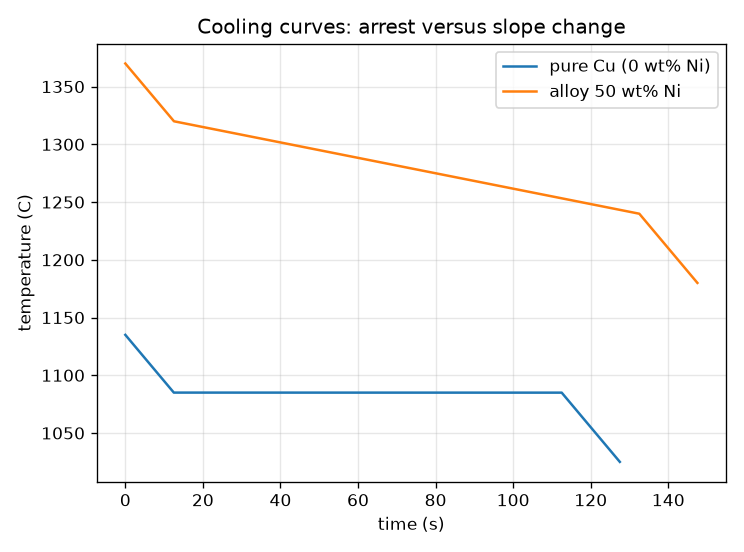
\includegraphics[width=0.85\linewidth]{figures/s01_cooling_curves.png}\\\small Pure copper holds a flat arrest; the 50 wt\% Ni alloy only bends.\end{center}

\subsection*{E. Worked example}
For the 50 wt\% Ni alloy find the melting range, say which phase region it is in at 1280 C, and compare how long the pure copper arrest lasts (L = 200 J/g, Q = 2 W/g).
\begin{enumerate}[nosep]
\item Read the diagram at 50 wt\% Ni: liquidus 1320 C, solidus 1240 C.
\item Melting range = 1320 - 1240 = 80 K.
\item At 1280 C we have 1240 \textless{} 1280 \textless{} 1320, so the alloy is liquid + solid.
\item Pure copper: the latent heat L = 200 J/g leaves at Q = 2 W/g, so the arrest lasts 200 / 2 = 100 s.
\item The alloy crosses its range in (0.5 * 80 + 200) / 2 = 120 s, an average rate of 80 / 120 = 0.67 K/s, against 2 / 0.5 = 4 K/s in the liquid.
\end{enumerate}
\textbf{Answer.} The melting range is 80 K, the alloy is liquid + solid at 1280 C, pure copper holds a 100 s arrest, and the alloy cools at 0.67 K/s through its range.

\subsection*{F. Questions}
\begin{enumerate}[nosep]
\item \textbf{Conceptual.} Why does a pure metal show a flat part on its cooling curve while an alloy only bends?
\item \textbf{Numerical.} How long does the 50 wt\% Ni alloy take to cool from 1320 C to 1240 C at Q = 2 W/g with c = 0.5 J/(g K) and L = 200 J/g? What is the mean cooling rate there?
\item \textbf{Graph and simulation interpretation.} On the cooling-curve view, where does the curve for 50 wt\% Ni change slope, and at which temperatures?
\item \textbf{Design and optimisation challenge.} Design: a brazing filler must be completely liquid at 1350 C and completely solid at 1200 C. Using this diagram, which Ni contents work (whole numbers)? Are pure Cu or pure Ni possible?
\end{enumerate}

\section{Session 2: Tie lines and the lever rule}

\subsection*{A. Real-world problem}
A foundry wants a casting that is exactly half liquid and half solid, a slurry that can be pressed into shape. At a given temperature the liquid and the solid in the band do not have the same composition as the alloy. How much of each is there, what is each made of, and which alloy and temperature give 50 percent liquid?

\subsection*{B. Concept and theory}
Take an alloy of overall composition C0 inside the two-phase band at temperature T. A horizontal tie line at T meets the liquidus at C\_L (the composition of the liquid) and the solidus at C\_S (the composition of the solid). The solute is conserved: the amount in the liquid plus the amount in the solid is the total, C0 = f\_L C\_L + f\_S C\_S with f\_L + f\_S = 1. Solving gives the lever rule: the fraction of a phase is the opposite arm of the tie line divided by the whole tie line. As the alloy cools, f\_L falls from 1 at the liquidus to 0 at the solidus, and the phase compositions slide along the two lines. The inverse problem has two ways to be posed: fix C0 and find T by solving f\_L = target, or fix T and find C0, which for a half-liquid alloy is the middle of the tie line.

\begin{itemize}[nosep]
\item C0: overall composition of the alloy (wt\% Ni)
\item C\_L: composition of the liquid at T (on the liquidus) (wt\% Ni)
\item C\_S: composition of the solid at T (on the solidus) (wt\% Ni)
\item f\_L, f\_S: mass fractions liquid and solid (no unit)
\item T: temperature of the tie line (C)
\end{itemize}

\begin{equation*}
C_0 = f_L\,C_L + f_S\,C_S,\qquad f_L+f_S=1
\end{equation*}

\begin{equation*}
f_L=\dfrac{C_S-C_0}{C_S-C_L},\qquad f_S=\dfrac{C_0-C_L}{C_S-C_L}
\end{equation*}

\begin{equation*}
f_L=\tfrac12\ \Rightarrow\ C_0=\dfrac{C_L+C_S}{2}
\end{equation*}

\begin{center}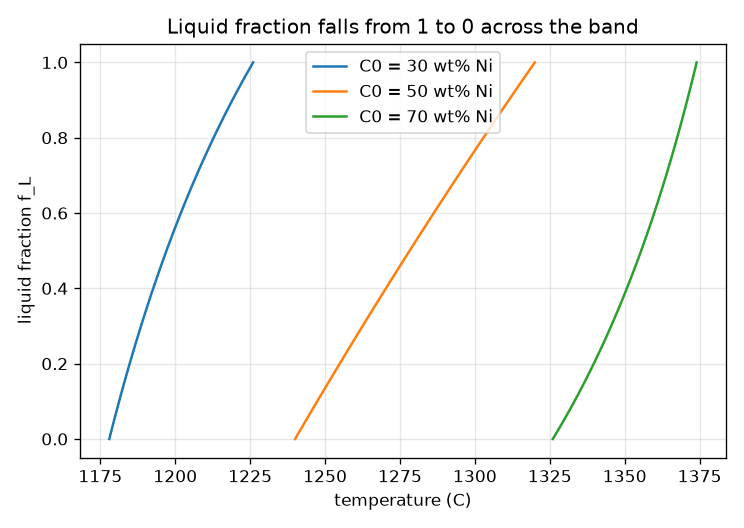
\includegraphics[width=0.85\linewidth]{figures/s02_liquid_fraction.png}\\\small Liquid fraction against temperature for three alloys.\end{center}

\subsection*{E. Worked example}
A 50 wt\% Ni alloy sits at 1300 C. Find the compositions of the liquid and the solid and the fraction that is liquid.
\begin{enumerate}[nosep]
\item Liquidus piece from (0, 1085) to (50, 1320): C\_L = 50 * (1300 - 1085) / (1320 - 1085) = 45.7 wt\% Ni.
\item Solidus piece from (50, 1240) to (100, 1455): C\_S = 50 + 50 * (1300 - 1240) / (1455 - 1240) = 64.0 wt\% Ni.
\item f\_L = (C\_S - C0) / (C\_S - C\_L) = (64.0 - 50) / (64.0 - 45.7) = 0.766 (76.6 percent liquid).
\item Check by mass balance: 0.766 * 45.7 + 0.234 * 64.0 = 50.0 wt\% Ni. It returns C0, as it must.
\end{enumerate}
\textbf{Answer.} The liquid is 45.7 wt\% Ni, the solid is 64.0 wt\% Ni, and 76.6 percent of the alloy is liquid.

\subsection*{F. Questions}
\begin{enumerate}[nosep]
\item \textbf{Conceptual.} Why is the liquid fraction given by the arm to the far end of the tie line (C\_S - C0) and not the near arm?
\item \textbf{Numerical.} For a 30 wt\% Ni alloy at 1200 C, find C\_L, C\_S and the liquid fraction.
\item \textbf{Graph and simulation interpretation.} On the liquid-fraction graph, which alloy of 30, 50 and 70 wt\% Ni has the widest temperature band? What does the steepness of a curve tell you?
\item \textbf{Design and optimisation challenge.} Design: at 1300 C which alloy composition is exactly half liquid? Which temperature makes a 50 wt\% Ni alloy half liquid? Give a second pair that works.
\end{enumerate}

\section{Session 3: Eutectic cooling, latent heat and fast freezing}

\subsection*{A. Real-world problem}
Electronics solder melts at a low temperature because tin and lead form a eutectic: a composition that melts lower than either metal. A factory joint may freeze in a fraction of a second, too fast for atoms to move as the lever rule assumes. The joint then contains a different structure than the diagram predicts, with a non-uniform composition inside each grain. How can we simulate the cooling curve, and when does equilibrium fail?

\subsection*{B. Concept and theory}
The illustrative lead-rich side has a liquidus falling from 327 C (pure Pb) to the eutectic at 183 C and 62 wt\% Sn, and an alpha solidus reaching 19 wt\% Sn at 183 C. Because both lines start at pure Pb, the ratio of solid to liquid composition on every tie line is constant, k = 19 / 62 = 0.306 (the partition coefficient). An alloy between 19 and 62 wt\% Sn first grows pro-eutectic alpha above 183 C, then the remaining liquid at 62 wt\% Sn freezes all at once at 183 C into the eutectic mixture. Cooling simulation: the heat content per gram H(T) = c T + L (1 - f\_s(T)), with f\_s the lever-rule solid fraction; heat leaves at rate q so H falls by q dt each step and the temperature is found by inverting H(T). The curve bends at the liquidus (the effective heat capacity is c + L \textbar{}df\_s/dT\textbar{}) and is flat during the eutectic arrest. Scheil freezing assumes no diffusion in the solid and a perfectly mixed liquid; mass balance gives C\_L = C0 f\_L\textasciicircum{}(k-1). The Clyne-Kurz model adds limited back-diffusion through alpha = D t\_f / lambda\textasciicircum{}2 and interpolates between Scheil and the lever rule.

\begin{itemize}[nosep]
\item C0: alloy composition (wt\% Sn)
\item k: partition coefficient, C\_solid / C\_liquid (19/62) (no unit)
\item f\_s, f\_L: solid and liquid fractions (no unit)
\item c: specific heat (0.2, illustrative) (J/(g K))
\item L: latent heat (50, illustrative) (J/g)
\item q: heat removal rate (W/g)
\item D: diffusion coefficient of Sn in solid alpha (1e-12, illustrative) (m\textasciicircum{}2/s)
\item lambda: half the dendrite arm spacing (20e-6, illustrative) (m)
\item t\_f: local freezing time (s)
\item alpha, a': back-diffusion parameters (no unit)
\end{itemize}

\begin{equation*}
f_s^{\text{pro}}=\dfrac{62-C_0}{62-19},\qquad f_{\text{eut}}=\dfrac{C_0-19}{62-19}\quad(19\le C_0\le 62)
\end{equation*}

\begin{equation*}
H(T)=c\,T+L\,\bigl(1-f_s(T)\bigr),\qquad H_{n+1}=H_n-q\,\Delta t,\qquad c_{\text{eff}}=c+L\left|\dfrac{df_s}{dT}\right|
\end{equation*}

\begin{equation*}
(1-f_s)\,dC_L=(1-k)\,C_L\,df_s\ \Rightarrow\ C_L=C_0\,f_L^{\,k-1},\quad C_S=k\,C_L
\end{equation*}

\begin{equation*}
f_{\text{eut}}^{\text{Scheil}}=\left(\dfrac{62}{C_0}\right)^{1/(k-1)}
\end{equation*}

\begin{equation*}
\alpha=\dfrac{D\,t_f}{\lambda^2},\quad a'=\alpha\left(1-e^{-1/\alpha}\right)-\tfrac12 e^{-1/(2\alpha)},\quad C_L=C_0\left[1-(1-2a'k)f_s\right]^{\frac{k-1}{1-2a'k}}
\end{equation*}

\begin{center}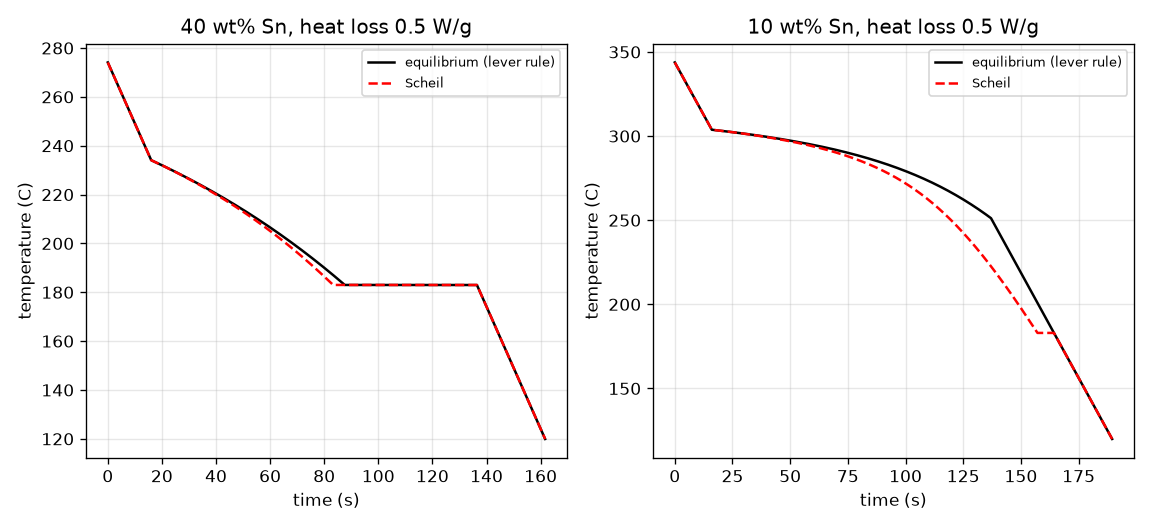
\includegraphics[width=0.85\linewidth]{figures/s03_cooling_curves.png}\\\small Simulated cooling curves: equilibrium (black) and Scheil (red dashed).\end{center}

\subsection*{E. Worked example}
A 40 wt\% Sn alloy is cooled at q = 0.5 W/g from 40 C above its liquidus. Find the liquidus, the fractions of pro-eutectic alpha and eutectic, the time to reach the liquidus and the length of the eutectic arrest.
\begin{enumerate}[nosep]
\item Liquidus: T\_L = 327 - (144 / 62) * 40 = 234.1 C.
\item Just above 183 C the lever rule with C\_L = 62 and C\_S = 19 gives pro-eutectic alpha = (62 - 40) / (62 - 19) = 0.512 (51.2 percent). The remaining liquid, 48.8 percent, becomes the eutectic mixture.
\item In the liquid the temperature falls at q / c = 0.5 / 0.2 = 2.5 K/s, so the first 40 C take c * 40 / q = 16 s.
\item At 183 C the latent heat of the remaining liquid leaves at constant temperature: the arrest lasts L * 0.488 / q = 50 * 0.488 / 0.5 = 48.8 s.
\item Check the simulation: it reproduces these times, its frozen fraction equals the lever rule between 234 and 183 C, and total heat removed equals c times the temperature drop plus L.
\end{enumerate}
\textbf{Answer.} Liquidus 234.1 C; 51.2 percent pro-eutectic alpha and 48.8 percent eutectic; 16 s to reach the liquidus; a 48.8 s eutectic arrest.

\subsection*{F. Questions}
\begin{enumerate}[nosep]
\item \textbf{Conceptual.} A 10 wt\% Sn alloy is single-phase alpha in the equilibrium diagram. Why does a fast-cooled joint of this alloy still contain some eutectic?
\item \textbf{Numerical.} Using the Scheil equation, find the liquid composition for a 10 wt\% Sn alloy when 90 percent has frozen, and then the fraction of eutectic it forms.
\item \textbf{Graph and simulation interpretation.} On the eutectic-versus-cooling-rate graph, at which cooling rates does the eutectic stay zero, and what limit does the curve approach at high rates?
\item \textbf{Design and optimisation challenge.} Design: choose the smallest whole-number Sn content whose liquid fraction is 60 percent at or below 230 C, and state the temperature. Why is the result not valid for fast-cooled solder?
\end{enumerate}

\section{Real-world mini-project}
\textbf{Choose a pasty solder: composition and working temperature.} A plumber's wiping solder must be 60 percent liquid when it is worked, and the working temperature must not exceed 230 C. Using the illustrative Pb-Sn-like diagram and the lever rule from Session 3 (\texttt{temperature\_for\_liquid\_fraction}), find the smallest whole-number tin content that meets both limits.

\section{The path ahead}
\begin{enumerate}[nosep]
\item \textbf{Session 4: Homogenising anneal.} A solid-state diffusion model across one dendrite arm with a heat treatment time.
\item \textbf{Session 5: Fit a diagram from cooling curves.} An inverse tool that reads simulated noisy cooling curves of several alloys and rebuilds the diagram.
\item \textbf{Session 6: Peritectic and intermetallic diagrams.} A second diagram type with a peritectic and a compound, with phase fractions on both sides of the line.
\item \textbf{Session 7: A moving freezing front.} A one-dimensional ingot with a heat-flow solver and the lever-rule enthalpy.
\item \textbf{Session 8: Quench and age: a heat treatment.} A quench-then-age calculation using a solvus line that falls with temperature.
\end{enumerate}

\section{Answers and hints}

\subsection*{Session 1}
\begin{enumerate}[nosep]
\item \textbf{Conceptual.} Hint: Where do the liquidus and solidus meet, and what does the latent heat have to do? Solution: A pure metal has liquidus = solidus, so all of the latent heat is released at a single temperature; the temperature cannot fall until it has all frozen, which gives a flat arrest. An alloy freezes over a range: only a little latent heat is released per degree, so the cooling is slowed (the curve bends to a lower slope) but never stops.
\item \textbf{Numerical.} Hint: Heat to remove = c times the temperature drop plus the latent heat L, then divide by Q. Solution: Heat = 0.5 * 80 + 200 = 240 J/g. Time = 240 / 2 = 120 s. Mean rate = 80 K / 120 s = 0.67 K/s. Sanity check: it is slower than the liquid rate Q/c = 4 K/s, as latent heat is being released.
\item \textbf{Graph and simulation interpretation.} Hint: Look for the two corners of the curve. Solution: It bends at 1320 C (the liquidus: first crystals, latent heat begins to be released, the curve flattens) and at 1240 C (the solidus: freezing is complete, the curve steepens again to the solid cooling rate). Between the two corners it falls more slowly but continuously, unlike pure copper whose curve is flat at 1085 C.
\item \textbf{Design and optimisation challenge.} Hint: Need liquidus \textless{}= 1350 and solidus \textgreater{}= 1200. Solve each with the straight line pieces. Solution: The solidus must be at least 1200 C: 1085 + 3.1 x \textgreater{}= 1200 gives x \textgreater{}= 37.1, so x \textgreater{}= 38. The liquidus must be at most 1350 C: 1320 + 2.7 (x - 50) \textless{}= 1350 gives x \textless{}= 61.1, so x \textless{}= 61. Alloys from 38 to 61 wt\% Ni work. Pure Cu is already liquid at 1200 C, pure Ni is still solid at 1350 C, so neither works. Trade-off: the middle of the window (about 50 wt\%) has the most margin in both limits. Assumption: the diagram is only illustrative.
\end{enumerate}

\subsection*{Session 2}
\begin{enumerate}[nosep]
\item \textbf{Conceptual.} Hint: Think of C0 sliding towards C\_L: what should the liquid fraction do? Solution: If C0 moves towards C\_L, the alloy is nearly all liquid, so f\_L must approach 1. The arm C\_S - C0 is then nearly the whole tie line and f\_L = (C\_S - C0)/(C\_S - C\_L) approaches 1. The lever balances like a seesaw: the phase whose composition is closer to C0 is the more plentiful, and its weight is the far arm.
\item \textbf{Numerical.} Hint: Read the compositions sideways: at 1200 C the liquidus piece is 0 to 50 wt\% Ni and the solidus piece is 0 to 50 wt\% Ni. Solution: C\_L = 50 * (1200 - 1085) / (1320 - 1085) = 24.5 wt\% Ni. C\_S = 50 * (1200 - 1085) / (1240 - 1085) = 37.1 wt\% Ni. f\_L = (37.1 - 30) / (37.1 - 24.5) = 0.562. Sanity check: 30 lies between 24.5 and 37.1, and is a little closer to the middle of the tie line than to the solid end, giving a fraction near one half.
\item \textbf{Graph and simulation interpretation.} Hint: Read the temperature where each curve starts at 1 and where it reaches 0. Solution: The 50 wt\% Ni alloy has the widest band, 80 K, because the liquidus and solidus are furthest apart there. A steep curve means the fraction changes quickly with temperature, so a small temperature change gives a large change in the amount of liquid; that is a poor choice for a process that needs a stable slurry.
\item \textbf{Design and optimisation challenge.} Hint: At fixed T, half liquid means C0 is the midpoint of the tie line. At fixed C0, solve f\_L = 0.5 for T. Solution: At 1300 C: C\_L = 45.7, C\_S = 64.0, so C0 = (45.7 + 64.0) / 2 = 54.8 wt\% Ni. For C0 = 50 wt\% Ni: half liquid at 1278.2 C. A second pair: 70 wt\% Ni at 1355.5 C, or at 1250 C and 1350 C the alloys 43.7 and 68.3 wt\% Ni. Trade-off: the higher the temperature, the more Ni is needed, and a steep f\_L curve means tight temperature control is needed.
\end{enumerate}

\subsection*{Session 3}
\begin{enumerate}[nosep]
\item \textbf{Conceptual.} Hint: Think about what happens to the Sn rejected by the first solid, and whether it can diffuse back. Solution: Each layer of solid that forms is poorer in Sn (k C\_L) than the liquid and rejects the extra Sn into the liquid. With fast cooling the Sn cannot diffuse back into the solid, so the liquid keeps getting richer in Sn until it reaches the eutectic composition, 62 wt\% Sn, and freezes as eutectic. The centre of each dendrite stays Sn-poor (coring) and the last liquid forms eutectic between dendrites.
\item \textbf{Numerical.} Hint: C\_L = C0 f\_L\textasciicircum{}(k-1) with k = 19/62 and f\_L = 0.1. For the eutectic set C\_L = 62. Solution: k - 1 = -0.6935. C\_L = 10 * 0.1\textasciicircum{}(-0.6935) = 49.4 wt\% Sn (between 10 and 62, as expected). The eutectic fraction is f\_L = (62 / 10)\textasciicircum{}(1/(k-1)) = 6.2\textasciicircum{}(-1.442) = 0.072, so 7.2 percent. The equilibrium diagram predicts 0 percent.
\item \textbf{Graph and simulation interpretation.} Hint: Read the plateau at slow rates and at fast rates. Solution: For a 10 wt\% Sn alloy the eutectic is 0 percent at slow rates (0.005 and 0.5 W/g, that is up to about 2.5 K/s in the liquid), appears as the rate rises (5.8 percent at 5 W/g) and approaches the Scheil limit of 7.2 percent (7.1 percent at 50 W/g). The reason: a high rate shortens the freezing time, so the diffusion parameter alpha falls and the solid behaves as if it could not exchange Sn at all.
\item \textbf{Design and optimisation challenge.} Hint: Use the lever rule between the liquidus and 183 C; find f\_L = 0.6 for several compositions. Solution: 30 wt\% Sn needs 230.6 C (too hot), 31 wt\% Sn needs 227.4 C, so 31 wt\% Sn is the smallest that works. This is an equilibrium result: fast heating or cooling of a real joint leaves more eutectic (35.1 percent against 25.6 percent for 30 wt\% Sn), which changes how much liquid there is at a given temperature. Treat the number as an illustration, not as a solder specification.
\end{enumerate}

\section{How to join}
Read \texttt{CONTRIBUTING.md} in the repository, then pick an issue labelled \texttt{good first issue}. Repository: \url{https://github.com/KrunalPanchal1995/openphasediagram}

\end{document}
